\chapter{Einsatzszenarien von reaktiver Programmierung}
\label{chap:scenario}
\section{Netflix}
Netflix ist maßgeblich bei der Entwicklung von RxJava beteiligt. Die Gründe für die Entwicklung von RxJava sind im Entwicklerblog \footnote{vgl. Christensen et al., Reactive Programming in the Netflix API with RxJava \cite{web:site:medium:netflix:reactive_programming}} des Unternehmens zu finden. Der wesentliche Grund für die Entwicklung war, dass Netflix die eigene API für nebenläufige Verarbeitung optimieren wollte. Das Problem von klassischen Lösungen wie z. B. Futures und Callbacks ist, dass diese Techniken nur für einen bestimmten Grad an Nebenläufigkeit sinnvoll ist. Futures können zwar verknüpft werden und über Callbacks ein blockierendes Warten vermeiden, allerdings nimmt die Lesbarkeit mit zunehmender Komplexität stark ab. Dies bezeichnet man als Callback Hell. Da die Programmierung mit Futures und Callbacks keine langfristige Lösung für hochgradig antwortbereite Systeme ist, implementierte das Entwicklerteam von Netflix die ReactiveX API für Java. 

\section{PayPal}
Die Firma Lightbend (Akka) fasst in ihrer Fallstudie\footnote{vgl. lightbend case studies paypal \cite{web:site:lightbend:case-studies:paypal}} den Technologiewechsel des Unternehmens PayPal zusammen.
PayPal nutzt für die Verarbeitung der Transaktionen die eigens entwickelte Plattform Squbs. Die Plattform ist in Scala geschrieben und nutzt das Akka Toolkit. Die Vorteile, die Paypal durch die neue Plattform hat, sind Geschwindigkeit und eine effizientere Auslastung der Hardware. Durch die hohe Geschwindigkeit können pro Tag bis zu einer Milliarde Transaktionen verarbeitet werden. Dies erreichen sie durch acht virtuelle Maschinen mit je zwei CPU-Kernen.

Ein weiterer Vorteil ist, dass der Code im Vergleich zur Java Implementierung um ca. 80\% reduziert wurde da Scala durch seine ausdrucksstarke Syntax den Code kürzt.

Für PayPal sind unter anderem das Aktorenmodell und die Streams Bibliothek die Schlüsseltechnologien um die hohen Lasten zu verarbeiten.

\section{Verizon}
Lightbend hat in einer Fallstudie\footnote{vgl. lightbend case studies verizon \cite{web:site:lightbend:case-studies:verizon} \label{casestudy:verizon}} den Technologiewechsel des Telekommunikationsunternehmens Verizon zusammengefasst. 
Verizon nutzt die reaktive Plattform von Lightbend (Akka u. v. m.) für ihr Onlineangebot und hat laut Angaben die Verkäufe verdoppelt. Die Performance der Software wurde bei halber Hardwareauslastung verdoppelt. Mit 2,5 Milliarden Transaktionen pro Jahr ist Verizon die  am sechsthäufigsten besuchte Website in den USA.

Das alte System basierte ursprünglich auf der Oracle Commerce Platform. Ein Problem war, dass das System eine monolithische Architektur hatte. Das heißt, dass die Codebase sehr komplex und groß war. Builds und Updates mussten über Nacht kompiliert werden. Die Testumgebungen für neue Features beanspruchten zwischen fünf und zehn Tagen an Vorbereitung. In Notfällen betrug die Zeit zum Einspielen der Fixes 24 Stunden. Trotz der Probleme nahm die Anzahl an Transaktionen und Neukunden zu. Das Entwicklerteam benötigte im Schnitt zwei Monate um neue Features zu veröffentlichen.

Verizon engagierte ein Team aus Softwarearchitekten zur Erkundung von neuen Technologien als Alternative zur Oracle Comerce Platform. Zur Auswahl standen Spring Boot und Lightbend's reaktive Plattform (Akka, Play u. v. m.). Das Team entschied sich für Lightbend's reaktive Plattform da sie technische Vorteile in asynchroner Verarbeitung und I/O bieten.

Die folgende Abbildung zeigt die Gegenüberstellung des alten und neuen Systems: 

\begin{figure}[H]
\caption{Gegenüberstellung des alten und neuen Systems}
\centering
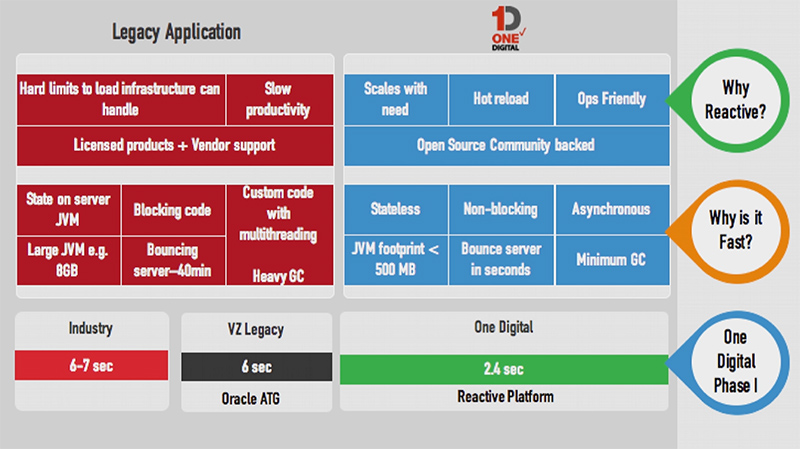
\includegraphics[scale=.5]{./media/verizon.jpg}
\footref{casestudy:verizon}
\end{figure}

Die starre Infrastruktur wurde durch eine skalierbare Infrastruktur ersetzt, die nach Bedarf Ressourcen bereitstellt. Das Entwicklungstempo wurde durch Hot Reload erhöht und ermöglicht eine insgesamt höhere Produktivität. Auf Lizenzen und Support wurde verzichtet und durch ein quelloffenes Backend ersetzt.

Die erhöhte Verarbeitungsgeschwindigkeit der Server wurde durch eine zustandlose, nicht blockierende und asynchrone Kommunikation erreicht. Der Speicherverbrauch wurde dadurch von 8 GB auf unter 500 MB gesenkt. Die Startzeit des Systems wurde von 40 Minuten auf wenige Sekunden gesenkt. Durch die Ersetzung der eigenen Multithreading Implementierung durch eine asynchrone Abstraktion wurde die Garbagecollection reduziert. 

Im direkten Performancevergleich sank die durchschnittliche Antwortzeit des neuen Systems von 6 Sekunden auf 2,4 Sekunden.

Die Verkäufe nahmen um 235\% zu und die \gls{Konversionsrate} stieg um 197\%. Aus technischer Sicht benötigt das neue System 40\% weniger Bauzeit und hat insgesamt 50\% weniger Kosten als das Vorgängersystem. 


